\chapter{1 Samuel 11}

\begin{figure}
  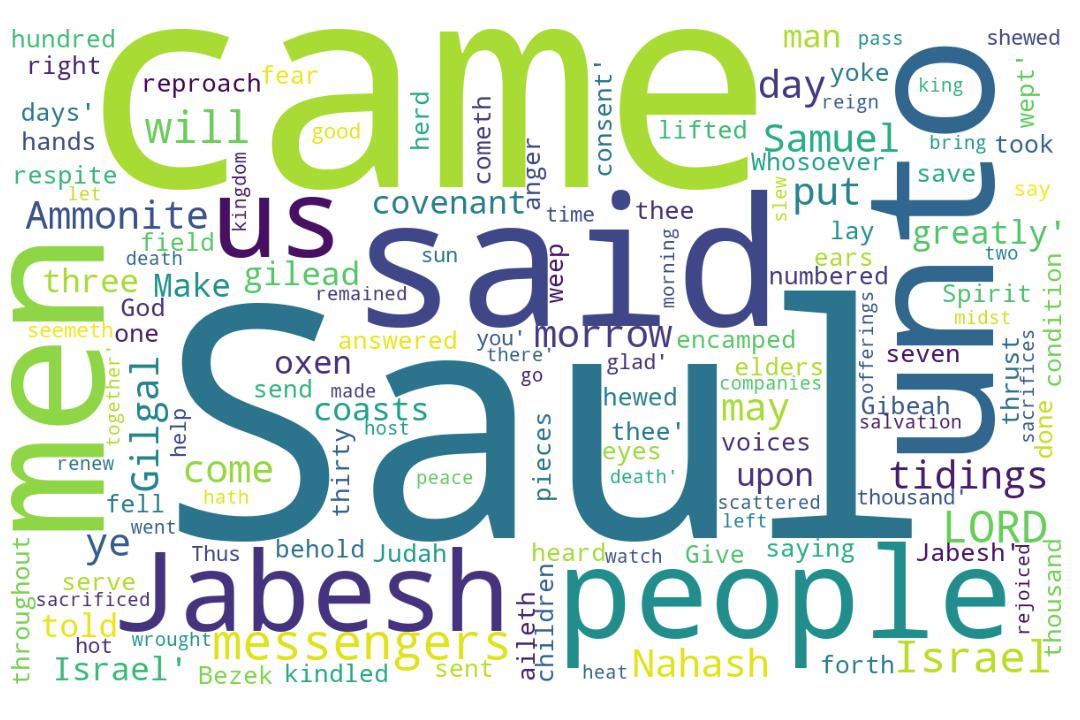
\includegraphics[width=\linewidth]{09OT-1Samuel/1Samuel11-WordCloud.jpg}
  \caption{1 Samuel 11 Word Cloud}
  \label{fig:1 Samuel 11 Word Cloud}
\end{figure}

\marginpar{\scriptsize \centering \fcolorbox{bone}{lime}{\textbf{WINNING THE BATTLE \& HEARTS}}\\ (1 Samuel 11:1--15) \begin{compactenum}[I.][8]
     \item The \textbf{Conditions for Peace} \index[scripture]{1 Samuel!1Sa 11:02} (1Sa 11:2) 
     \item A \textbf{Proposed Covenant}  \index[scripture]{1 Samuel!1Sa 11:02} (1Sa 11:2) 
     \item  \textbf{Cut in Pieces}  \index[scripture]{1 Samuel!1Sa 11:07} (1Sa 11:7) 
     \item The \textbf{Purposed Consent}  \index[scripture]{1 Samuel!1Sa 11:07} (1Sa 11:7) 
     \item Three \textbf{Companies of People}  \index[scripture]{1 Samuel!1Sa 11:11} (1Sa 11:11) 
     \item What \textbf{Came to Pass}  \index[scripture]{1 Samuel!1Sa 11:11} (1Sa 11:11) 
     \item  \textbf{Commemorating Peace}  \index[scripture]{1 Samuel!1Sa 11:15} (1Sa 11:15) 
%    \begin{compactenum}[A.]
%    	\item Result of Undeterred Sin

%    \end{compactenum}
\end{compactenum}}

\footnote{\textcolor[cmyk]{0.99998,1,0,0}{\hyperlink{TOC}{Return to end of Table of Contents.}}}\footnote{\href{https://audiobible.com/bible/1_samuel_11.html}{\textcolor[cmyk]{0.99998,1,0,0}{1 Samuel 11 Audio}}}\textcolor[cmyk]{0.99998,1,0,0}{Then Nahash the Ammonite came up, and encamped against \fcolorbox{bone}{MYGOLD}{Jabesh-gilead}: and all the men of Jabesh said unto Nahash, Make a covenant with us, and we will serve thee.}
[2] \textcolor[cmyk]{0.99998,1,0,0}{And Nahash the Ammonite answered them, On this \fcolorbox{bone}{lime}{\emph{condition}} will I make \emph{a} \fcolorbox{bone}{lime}{\emph{covenant}} with you, that I may thrust out all your right eyes, and lay it \emph{for} a reproach upon all Israel.}
[3] \textcolor[cmyk]{0.99998,1,0,0}{And the elders of Jabesh said unto him, Give us seven days' respite, that we may send messengers unto all the coasts of Israel: and then, if \emph{there} \emph{be} no man to save us, we will come out to thee.}\\
\\
\P \textcolor[cmyk]{0.99998,1,0,0}{Then came the messengers to Gibeah of Saul, and told the tidings in the ears of the people: and all the people lifted up their voices, and wept.}
[5] \textcolor[cmyk]{0.99998,1,0,0}{And, behold, Saul came after the herd out of the field; and Saul said, What \emph{aileth} the people that they weep? And they told him the tidings of the men of Jabesh.}
[6] \textcolor[cmyk]{0.99998,1,0,0}{And the Spirit of God came upon Saul when he heard those tidings, and his anger was kindled greatly.}
[7] \textcolor[cmyk]{0.99998,1,0,0}{And he took a yoke of oxen, and hewed them in \fcolorbox{bone}{lime}{pieces}, and sent \emph{them} throughout all the coasts of Israel by the hands of messengers, saying, Whosoever cometh not forth after Saul and after Samuel, so shall it be done unto his oxen. And the fear of the LORD fell on the people, and they came out with one \fcolorbox{bone}{lime}{consent}.}
[8] \textcolor[cmyk]{0.99998,1,0,0}{And when he numbered them in Bezek, the children of Israel were three hundred thousand, and the men of Judah thirty thousand.}
[9] \textcolor[cmyk]{0.99998,1,0,0}{And they said unto the messengers that came, Thus shall ye say unto the men of \fcolorbox{bone}{MYGOLD}{Jabesh-gilead}, To morrow, by \emph{that} \emph{time} the sun be hot, ye shall have help. And the messengers came and shewed \emph{it} to the men of Jabesh; and they were glad.}
[10] \textcolor[cmyk]{0.99998,1,0,0}{Therefore the men of Jabesh said, To morrow we will come out unto you, and ye shall do with us all that seemeth good unto you.}
[11] \textcolor[cmyk]{0.99998,1,0,0}{And it was \emph{so} on the morrow, that Saul put the people in three \fcolorbox{bone}{lime}{companies}; and they came into the midst of the host in the morning watch, and slew the Ammonites until the heat of the day: and it \fcolorbox{bone}{lime}{came to pass}, that they which remained were scattered, so that two of them were not left together.}\\
\\
\P \textcolor[cmyk]{0.99998,1,0,0}{And the people said unto Samuel, Who \emph{is} he that said, Shall Saul reign over us? bring the men, that we may put them to death.}
[13] \textcolor[cmyk]{0.99998,1,0,0}{And Saul said, There shall not a man be put to death this day: for to day the LORD hath wrought salvation in Israel.}
[14] \textcolor[cmyk]{0.99998,1,0,0}{Then said Samuel to the people, Come, and let us go to Gilgal, and renew the kingdom there.}
[15] \textcolor[cmyk]{0.99998,1,0,0}{And all the people went to Gilgal; and there they made Saul king before the LORD in Gilgal; and there they sacrificed sacrifices of \fcolorbox{bone}{lime}{peace} offerings before the LORD; and there Saul and all the men of Israel rejoiced greatly.}